%Este trabalho está licenciado sob a Licença Creative Commons Atribuição-CompartilhaIgual 3.0 Não Adaptada. Para ver uma cópia desta licença, visite http://creativecommons.org/licenses/by-sa/3.0/ ou envie uma carta para Creative Commons, PO Box 1866, Mountain View, CA 94042, USA.

%\documentclass[main.tex]{subfiles}
%\begin{document}

\chapter{Aproximação de funções}\index{aproximação!de funções}

O problema geral de interpolação pode ser definido como:

%Sejam    $\mathcal{F}$ uma família de funções $f:D\to E$ e $\left\{(x_i,y_i)\right\}_{i=1}^N$ um conjunto de pares ordenados tais que $x_i\in D$ e $y_i\in E$, encontrar uma função $f$ da família dada tal que $f(x_i)=y_i$ para cada $1\leq i \leq N$.

Seja $\left\{(x_i,y_i)\right\}_{i=1}^n$ um conjunto de pares ordenados tais que $x_i \ne x_j$ se $i=j$, encontre  uma função $f \in \mathcal{F}$ (uma família de funções) tal que
$$f(x_i)=y_i, \;\;\; i=1,...,n$$

\begin{ex} Encontrar uma função $f(x)$ da forma $f(x)=a e^{bx}$ onde $a$ e $b$ são constantes tal que $f(1)=1$ e $f(2)=5$. Este problema equivale a resolver o seguinte sistema de equações:
\begin{eqnarray*}
ae^b&=&1\\
ae^{2b}&=&5
\end{eqnarray*}
Dividindo a segunda equação pela primeira, temos $e^b=5$, logo, $b=\ln(5)$. Substituindo este valor em qualquer das equações, temos $a=\frac{1}{5}$. Assim $$f(x)=\frac{1}{5}e^{\ln(5) x}=\frac{1}{5}5^x=5^{x-1}.$$
\end{ex}

\begin{ex} Encontrar a função polinomial do tipo $f(x)=a+bx+cx^2$ que passe pelos pontos $(-1,2)$, $(0,1)$, $(1,6)$. Observamos que podemos encontrar os coeficientes $a$, $b$ e $c$ através do seguinte sistema linear:
\begin{eqnarray*}
a-b+c&=&2\\
a&=&1\\
a+b+c&=&6
\end{eqnarray*}
cuja solução é dada por $a=1$, $b=2$ e $c=3$. Portanto $$f(x)=1+2x+3x^2.$$
\end{ex}

\section{Interpolação polinomial}\index{interpolação!polinomial}

Interpolação polinomial é o caso particular do problema geral de interpolação quando a família de funções é constituída de polinômios.

\begin{teo}\label{teo_interp_poli} Seja $\{(x_i,y_i)\}_{i=1}^{n}$ um conjunto de $n$ pares ordenados de números reais tais que $x_i \ne x_j$ se $i=j$.
Existe um único polinômio $p(x)$ de grau $n-1$ ou inferior que passa por todos os pontos dados.
\end{teo}
\begin{proof} Observe que o problema de encontrar os coeficientes $a_1$, $a_2$,\ldots, $a_n$ do polinômio
$$p(x)=a_1+a_2x+a_3x^2+\cdots a_nx^{n-1}=\sum_{k=1}^n a_k x^{k-1}$$
tal que $p(x_i)=y_i$ é equivalente a resolver o sistema linear com $n$ equações e $n$ incógnitas:
\begin{eqnarray*}
a_1+a_2x_1+a_3x_1^2+\cdots +a_n x_1^{n-1}&=&y_1\\
a_1+a_2x_2+a_3x_2^2+\cdots +a_n x_2^{n-1}&=&y_2\\
&\vdots&\\
a_1+a_2x_n+a_3x_n^2+\cdots +a_n x_n^{n-1}&=&y_n
\end{eqnarray*}
que pode ser escrito na forma matricial como
$$\begin{bmatrix}
1 & x_1 & x_1^2 & \cdots & x_1^{n-1}\\
1 & x_2 & x_2^2 & \cdots & x_2^{n-1}\\
1 & x_3 & x_3^2 & \cdots & x_3^{n-1}\\
\vdots&\vdots&\vdots&\ddots&\vdots\\
1 & x_n & x_n^2 & \cdots & x_n^{n-1}
\end{bmatrix}
\begin{bmatrix}
a_1\\a_2\\a_3\\ \vdots \\a_n
\end{bmatrix}=
\begin{bmatrix}
y_1\\y_2\\y_3\\ \vdots \\y_n
\end{bmatrix}
$$
A matriz envolvida é uma matriz de Vandermonde de ordem $n$ cujo determinante é dado por
$$\prod_{1\leq i<j\leq n}\left(x_j-x_i\right)$$
É fácil ver que se as abscissas são diferentes dois a dois, então o determinante é não-nulo. Disto decorre que o sistema possui uma solução e que esta solução é única.
\end{proof}

\begin{ex} Encontre o polinômio da forma $p(x)=a_1+a_2x+a_3x^2+a_4x^3$ que passa pelos pontos
$$(0,1),(1,2),(2,4),(3,8).$$

Para encontrar os coeficientes devemos resolver o sistema linear
\begin{eqnarray*}
a_1                &=&1\\
a_1+ a_2+ a_3+  a_4&=&2\\
a_1+2a_2+4a_3+ 8a_4&=&4\\
a_1+3a_2+9a_3+27a_4&=&8
\end{eqnarray*}
cuja solução é $a_1=1$, $a_2=\frac{5}{6}$, $a_3=0$ e $a_4=\frac{1}{6}$. Portanto
$$p(x)=1+\frac{5}{6}x+\frac{1}{6}x^3$$
\end{ex}

% \begin{ex} Encontre o polinômio da forma $P(x)=a_0+a_1x+a_2x^2+a_3x^3$ que passa pelos pontos
% $$(0,0),(1,1),(2,4),(3,9)$$
% Este problema é equivalente ao seguinte sistema linear:
% \begin{eqnarray*}
% a_0&=&0\\
% a_0+a_1+a_2+a_3&=&1\\
% a_0+2a_1+4a_2+8a_3&=&4\\
% a_0+3a_1+9a_2+27a_3&=&9
% \end{eqnarray*}
% cuja solução é $a_0=0$, $a_1=0$, $a_2=1$ e $a_3=0$. Portanto
% $$P(x)=x^2$$
% \end{ex}

Esta abordagem direta que fizemos ao calcular os coeficientes do polinômio na base canônica se mostra ineficiente quando o número de pontos é grande e quando existe grande discrepância nas abscissas. Neste caso a matriz de Vandermonde é mal-condicionada (ver \cite{Gautschi}), acarretando um aumento dos erros de arredondamento na solução do sistema.

Uma maneira de resolver este problema é escrever o polinômio em uma base que produza um sistema bem-condicionado.

\section{Diferenças divididas de Newton}\index{diferenças divididas de Newton}
O método das diferenças divididas de Newton consiste em construir o polinômio interpolador da forma
\begin{eqnarray*}
p(x) &=& a_1 + a_2 (x-x_1) + a_3 (x-x_1)(x-x_2) + \cdots \\
     &+& a_n (x-x_1)(x-x_2)\cdots (x-x_{n-1}).
\end{eqnarray*}
Podemos encontrar os coeficientes $a_i$ resolvendo o sistema linear
\begin{small}
\begin{eqnarray*}
&a_1               &= y_1\\
&a_1+a_2(x_2-x_1)  &= y_2\\
&a_1+a_2(x_3-x_1)+a_3(x_3-x_1)(x_3-x_2) &= y_3\\
&\vdots&\\
&a_1+a_2(x_n-x_1)+\cdots + a_n(x_n-x_1)\cdots (x_n-x_{n-1}) &= y_n
\end{eqnarray*}
\end{small}
que pode ser escrito na forma matricial como
\begin{small}
  \begin{equation*}
    \begin{bmatrix}
      1& 0        & 0   & \!\cdots\!&0\\
      1&(x_2-x_1) & 0 &\!\cdots\!&0\\
      1&(x_3-x_1) &(x_3-x_1)(x_3-x_2) &\!\cdots\!&0\\
      \vdots&\vdots&\vdots&\!\ddots\!&\vdots\\
      1&(x_n-x_1) &(x_n-x_1)(x_n-x_2) &\!\cdots\!& (x_n-x_1)\cdots(x_n-x_{n-1})\\
    \end{bmatrix}\begin{bmatrix}
      a_1\\a_2\\a_3\\ \vdots \\a_n
    \end{bmatrix} = 
    \begin{bmatrix}
      y_1\\y_2\\y_3\\ \vdots \\y_n
    \end{bmatrix}
  \end{equation*}
\end{small}

Este é um sistema triangular inferior que pode ser facilmente resolvido conforme:
\begin{eqnarray*}
a_1&=&y_1\\
a_2&=&\frac{y_2-a_1}{x_2-x_1}=\frac{y_2-y_1}{x_2-x_1}\\
a_3&=&\frac{y_3-a_2(x_3-x_1)-a_1}{(x_3-x_1)(x_3-x_2)}=\frac{\frac{y_3-y_2}{(x_3-x_2)}-\frac{y_2-y_1}{(x_2-x_1)}}{(x_3-x_1)}\\
&\ldots&
\end{eqnarray*}
A solução deste sistema pode ser escrita em termos das Diferenças Divididas de Newton, definidas recursivamente conforme:
\begin{eqnarray*}
f[x_j]&=&y_j\\
f[x_j,x_{j+1}]&=&\frac{f[x_{j+1}]-f[x_j]}{x_{j+1}-x_j}\\
f[x_j,x_{j+1},x_{j+2}]&=&\frac{f[x_{j+1},x_{j+2}]-f[x_j,x_{j+1}]}{x_{j+2}-x_j}\\
&\vdots&
\end{eqnarray*}
Nesta notação, temos
$a_k=f[x_1,x_2,\ldots,x_k]$

Podemos esquematizar o método na seguinte tabela:
$$
\begin{array}{|c|c|c|c|c|}\hline
j &x_j&f[x_j]&f[x_{j-1},x_j]&f[x_{j-2},x_{j-1},x_j]\\\hline
1 & x_1 & f[x_1]&&\\
&&&f[x_1,x_2]=\frac{f[x_2]-f[x_1]}{x_2-x_1}&\\
2 & x_2&f[x_2]&&f[x_1,x_2,x_3]=\frac{f[x_2,x_3]-f[x_1,x_2]}{x_3-x_1}\\
&&&f[x_2,x_3]=\frac{f[x_3]-f[x_2]}{x_3-x_2}&\\
3 & x_2&f[x_2]&&\\\hline
\end{array}
$$

\begin{ex}
Encontrar o polinômio que passe pelos seguintes pontos
$$(-1,3),(0,1),(1,3),(3,43)$$

\begin{equation*}
\begin{array}{|c||c|c|c|c|c|}\hline
 j&x_j&f[x_j]&f[x_{j-1},x_j]&f[x_{j-2},x_{j-1},x_j]&f[x_{j-3},x_{j-2},x_{j-1},x_j]\\\hline
1& -1 & 3&&&\\
&&&\frac{1-3}{0-(-1)}=-2&&\\
2&0&1&&\frac{2-(-2)}{1-(-1)}=2&\\
&&&\frac{3-1}{1-0}=2&&\frac{6-2}{3-(-1)}=1\\
3&1&3&&\frac{20-2}{3-0}=6&\\
&&&\frac{43-3}{3-1}=20&&\\
4&3&43&&&\\\hline
\end{array}  
\end{equation*}



Portanto
\begin{eqnarray*}
P(x)&=&3-2(x+1)+2(x+1)x+(x+1)x(x-1)\\
&=&x^3+2x^2-x+1
\end{eqnarray*}
\end{ex}

\subsection*{Exercícios}


\begin{Exercise}\label{exer:interp1}
Considere o seguinte conjunto de pontos: $$(-2,-47),(0,-3),(1,4)(2,41)$$. Encontre o polinômio interpolador usando os métodos vistos. 
\end{Exercise}
\begin{Answer}
  \begin{tiny}
$5x^3+2x-3$    
  \end{tiny}
\end{Answer}

\ifisscilab
\begin{Exercise}
  No \verb+Scilab+, faça um gráfico com os pontos e o polinômio interpolador do Exercício~\ref{exer:interp1}.
\end{Exercise}
\fi

\section{Polinômios de Lagrange}\index{polinômios!de Lagrange}
Outra maneira clássica de resolver o problema da interpolação polinomial é através dos polinômios de Lagrange. Dado um conjunto de pontos $\{x_j\}_{j=1}^n$ distintos dois a dois, definimos os polinômios de Lagrange como os polinômios de grau $n-1$ que satisfazem
$$
L_k(x_j)=\left\{\begin{array}{rl}
1,& \text{se }k=j\\
0,& \text{se }k\neq j
\end{array}
\right.
$$
Assim, o polinômio de grau $n-1$ que interpola os pontos dados, tais $p(x_j)=y_j, j=1,\ldots,n$ é dado por
$$p(x)=y_1L_1(x)+y_2L_2(x)+\cdots +y_nL_n(x)=\sum_{k=1}^n y_k L_k(x)$$

Para construir os polinômios de Lagrange, podemos analisar a sua forma fatorada, ou seja:
$$L_k(x)=c_k\prod_{\substack{j=1\\j\ne i}}^{n} (x-x_j)$$
onde o coeficiente $c_k$ é obtido da condição $L_k(x_k)=1$:
$$L_k(x_k)=c_k\prod_{\substack{j=1\\j\ne i}}^{n} (x_k-x_j) \Longrightarrow  c_k=\frac{1}{\displaystyle \prod_{\substack{j=1\\j\ne i}}^{n} (x_k-x_j)}$$
Portanto,
$$L_k(x)=\prod_{\substack{j=1\\j\ne i}}^{n} \frac{(x-x_j)}{(x_k-x_j)}$$

\begin{obs} O problema de interpolação quando escrito usando como base os polinômios de Lagrange produz um sistema linear diagonal.
\end{obs}

\begin{ex}Encontre o polinômio da forma $p(x)=a_1+a_2x+a_3x^2+a_4x^3$ que passa pelos pontos
$$(0,0),(1,1),(2,4),(3,9)$$
Escrevemos:
\begin{eqnarray*}
L_1(x)&=& \frac{(x-1)(x-2)(x-3)}{(0-1)(0-2)(0-3)}=-\frac{1}{6}x^3+x^2-\frac{11}{6}x+1\\
L_2(x)&=& \frac{x(x-2)(x-3)}{1(1-2)(1-3)}=\frac{1}{2}x^3-\frac{5}{2}x^2+3x\\
L_3(x)&=& \frac{x(x-1)(x-3)}{2(2-1)(2-3)}=-\frac{1}{2}x^3+2x^2-\frac{3}{2}x\\
L_4(x)&=& \frac{x(x-1)(x-2)}{3(3-1)(3-2)}=\frac{1}{6}x^3-\frac{1}{2}x^2+\frac{1}{3}x
\end{eqnarray*}
Assim temos:
$$P(x)=0\cdot L_1(x)+1\cdot L_2(x)+4\cdot L_3(x)+9\cdot L_4(x)=x^2$$
\end{ex}

\begin{ex}Encontre o polinômio da forma $p(x)=a_1+a_2x+a_3x^2+a_4x^3$ que passa pelos pontos
$$(0,0),(1,1),(2,0),(3,1)$$
Como as abscissas são as mesmas do exemplo anterior, podemos utilizar os mesmos polinômios de Lagrange, assim temos:
$$p(x)=0\cdot L_1(x)+1\cdot L_2(x)+0\cdot L_3(x)+1\cdot L_4(x)=\frac{2}{3}x^3-3x^2+\frac{10}{3}x$$
\end{ex}

\section{Aproximação de funções reais por polinômios interpoladores}\index{aproximação!de funções!por polinômios}

\begin{teo}\label{teo_interp}
Dados $n+1$ pontos distintos, $x_0,\ x_1,\ \cdots,\ x_n$, dentro de um intervalo $[a,b]$ e uma função $f$ com $n+1$ derivadas contínuas nesse intervalo ($f\in C^{n+1}[a,b]$), então para cada $x$ em $[a,b]$, existe um número $\xi(x)$ em $(a,b)$ tal que
$$
f(x)=P(x)+\frac{f^{(n+1)}(\xi(x))}{(n+1)!}(x-x_0)(x-x_1)\cdots(x-x_n),
$$
onde $P(x)$ é o polinômio interpolador. Em especial, pode-se dizer que
$$
|f(x)-P(x)|\leq \frac{M}{(n+1)!}\left|(x-x_0)(x-x_1)\cdots(x-x_n)\right|,
$$
onde
$$
M=\max_{x\in[a,b]}|f^{(n+1)}(\xi(x))|
$$
\end{teo}

\begin{ex}
Considere a função $f(x)=\cos(x)$ e o polinômio $P(x)$ de grau 2 tal que $P(0)=\cos(0)=1$, $P(\frac{1}{2})=\cos(\frac{1}{2})$ e $P(1)=\cos(1)$. Use a fórmula de Lagrange para encontrar $P(x)$. Encontre o erro máximo que se assume ao aproximar o valor de $\cos(x)$ pelo de $P(x)$ no intervalo $[0,1]$. Trace os gráficos de $f(x)$ e $P(x)$ no intervalo $[0,1]$ no mesmo plano cartesiano e, depois, trace o gráfico da diferença $\cos(x)-P(x)$. Encontre o erro efetivo máximo $|\cos(x)-P(x)|$.
\end{ex}

\begin{eqnarray*}
P(x)&=&1\frac{(x-\frac{1}{2})(x-1)}{(0-\frac{1}{2})(0-1)}+\cos\left(\frac{1}{2}\right)\frac{(x-0)(x-1)}{(\frac{1}{2}-0)(\frac{1}{2}-1)}+\cos(1)\frac{(x-0)(x-\frac{1}{2})}{(1-0)(1-\frac{1}{2})}\\
&\approx&   1 - 0,0299720583066x - 0,4297256358252x^2
\end{eqnarray*}

\ifisscilab
\begin{verbatim}
L1=poly([.5 1],'x');L1=L1/horner(L1,0)
L2=poly([0 1],'x');L2=L2/horner(L2,0.5)
L3=poly([0 .5],'x');L3=L3/horner(L3,1)
P=L1+cos(.5)*L2+cos(1)*L3
x=[0:.05:1]
plot(x,cos)
plot(x,horner(P,x),'red')
plot(x,horner(P,x)-cos(x))
\end{verbatim}
\fi

Para encontrar o erro máximo, precisamos estimar $|f'''(x)|=|\sin(x)|\leq \sin(1)<0,85$ e
$$
\max_{x\in[0,1]} \left|x\left(x-\frac{1}{2}\right)(x-1)\right|
$$
O polinômio de grau três $Q(x)=x\left(x-\frac{1}{2}\right)(x-1)$ tem um mínimo (negativo) em $x_1=\frac{3+\sqrt{3}}{6}$ e um máximo (positivo) em $x_2=\frac{3-\sqrt{3}}{6}$. Logo:
$$
\max_{x\in[0,1]} \left|x\left(x-\frac{1}{2}\right)(x-1)\right|\leq \max\{|Q(x_1)|,\ |Q(x_2)|\}\approx 0,0481125.
$$
Portanto:
$$
|f(x)-P(x)|< \frac{0,85}{3!}0,0481125\approx 0,0068159<7\cdot 10^{-3}
$$

Para encontrar o erro efetivo máximo, basta encontrar o máximo de $|P(x)-cos(x)|$. O mínimo (negativo) de $P(x)-cos(x)$ acontece em $x_1=4,29\cdot 10^{-3}$ e o máximo (positivo) acontece em $x_2=3,29\cdot 10^{-3}$. Portanto, o erro máximo efetivo é $4,29\cdot 10^{-3}$.

\begin{ex}\label{exemp_simpson}
Considere o problema de aproximar o valor da integral $\int_0^1 f(x)dx$ pelo valor da integral do polinômio $P(x)$ que coincide com $f(x)$ nos pontos $x_0=0$, $x_1=\frac{1}{2}$ e $x_2=1$. Use a fórmula de Lagrange para encontrar $P(x)$. Obtenha o valor de $\int_0^1f(x)dx$ e encontre uma expressão para o erro de truncamento.
\end{ex}
O polinômio interpolador de $f(x)$ é
\begin{eqnarray*}
P(x)&=&f(0)\frac{(x-\frac{1}{2})(x-1)}{(0-\frac{1}{2})(0-1)}+f\left(\frac{1}{2}\right)\frac{(x-0)(x-1)}{(\frac{1}{2}-0)(\frac{1}{2}-1)}+f(1)\frac{(x-0)(x-\frac{1}{2})}{(1-0)(1-\frac{1}{2})}\\
&=&   f(0)(2x^2-3x+1)+f\left(\frac{1}{2}\right)(-4x^2+4x)+f(1)(2x^2-x)
\end{eqnarray*}
e a integral de $P(x)$ é:
\begin{eqnarray*}
\int_0^1 P(x)dx &=& \left[f(0)\left(\frac{2}{3}x^3 - \frac{3}{2}x^2+x\right)\right]_0^1 + \left[f\left(\frac{1}{2}\right)\left(-\frac{4}{3}x^3+2x^2\right)\right]_0^1 \\
&+& \left[f(1)\left(\frac{2}{3}x^3-\frac{1}{2}x^2\right)\right]_0^1\\
&=& f(0)\left(\frac{2}{3}-\frac{3}{2}+1\right)+f\left(\frac{1}{2}\right)\left(-\frac{4}{3}+2\right)+f(1)\left(\frac{2}{3}-\frac{1}{2}\right)\\
&=& \frac{1}{6}f(0)+\frac{2}{3}f\left(\frac{1}{2}\right)+\frac{1}{6}f(1)
\end{eqnarray*}
Para fazer a estimativa de erro usando o Teorema~\ref{teo_interp}, e temos
\begin{eqnarray*}
\left|\int_0^1f(x)dx-\int_0^1 P(x)dx\right|&=&\left|\int_0^1f(x)- P(x)dx\right|\\
&\leq&\int_0^1|f(x)- P(x)|dx\\
&\leq& \frac{M}{6}  \int_0^1\left|x\left(x-\frac{1}{2}\right)(x-1)\right|dx\\
&=& \frac{M}{6}  \left[\int_0^{1/2}x\left(x-\frac{1}{2}\right)(x-1)dx\right.\\
&-&\left.\int_{1/2}^1x\left(x-\frac{1}{2}\right)(x-1)dx\right]\\
&=& \frac{M}{6}  \left[\frac{1}{64}-\left(-\frac{1}{64}\right)\right]=\frac{M}{192}.
\end{eqnarray*}
Lembramos que $M=\max_{x\in[0,1]}|f'''(x)|$.

\begin{obs}Existem estimativas melhores para o erro de truncamento para este esquema de integração numérica. Veremos com mais detalhes tais esquemas na teoria de integração numérica.
\end{obs}

\begin{ex}
Use o resultado do exemplo anterior para aproximar o valor das seguintes integrais:\\

a) $\displaystyle \int_0^1 \ln(x+1) dx$\\

b) $\displaystyle \int_0^1 e^{-x^2}dx$

\end{ex}
\begin{sol}
Usando a fórmula obtida, temos que
$$
\int_0^1\ln(x+1) dx \approx 0,39\pm \frac{1}{96}
$$
$$
\int_0^1 e^{-x^2} dx \approx 0,75\pm \frac{3,87}{192}
$$  
\end{sol}

\subsection*{Exercícios}

\begin{Exercise}
  Use as mesmas técnicas usadas o resultado do Exemplo~\ref{exemp_simpson} para obter uma aproximação do valor de:
  \begin{equation*}
    \int_0^1 f(x)dx
  \end{equation*}
através do polinômio interpolador que coincide com $f(x)$ nos pontos $x=0$ e $x=1$.
\end{Exercise}
\begin{Answer}
  \begin{tiny}
  $\int_0^1 P(x)dx =\frac{f(0)+f(1)}{2}$, $\frac{1}{12}\max_{x\in[0,1]}|f''(x)|$  
  \end{tiny}
\end{Answer}



\section{Ajuste de curvas}\index{método!dos mínimos quadrados}\index{ajuste de curvas}

% No problema de interpolação, desejamos encontrar uma função $f(x)$ tal que
% $$f(x_j)=y_j$$
% para um conjunto de pontos dados.
\begin{defn}
O problema de \emph{ajuste de curvas} consiste em dado um conjunto de $N$ pontos $(x_j,y_j)$, encontre a função $f(x)$ de uma família de funções que melhor aproxima os pontos dados.
\end{defn}

Por exemplo, dado um conjunto de $15$ pontos como na figura \ref{minquad} encontre a reta que melhor se ajusta aos pontos.
\begin{figure}[htp]
\begin{center}
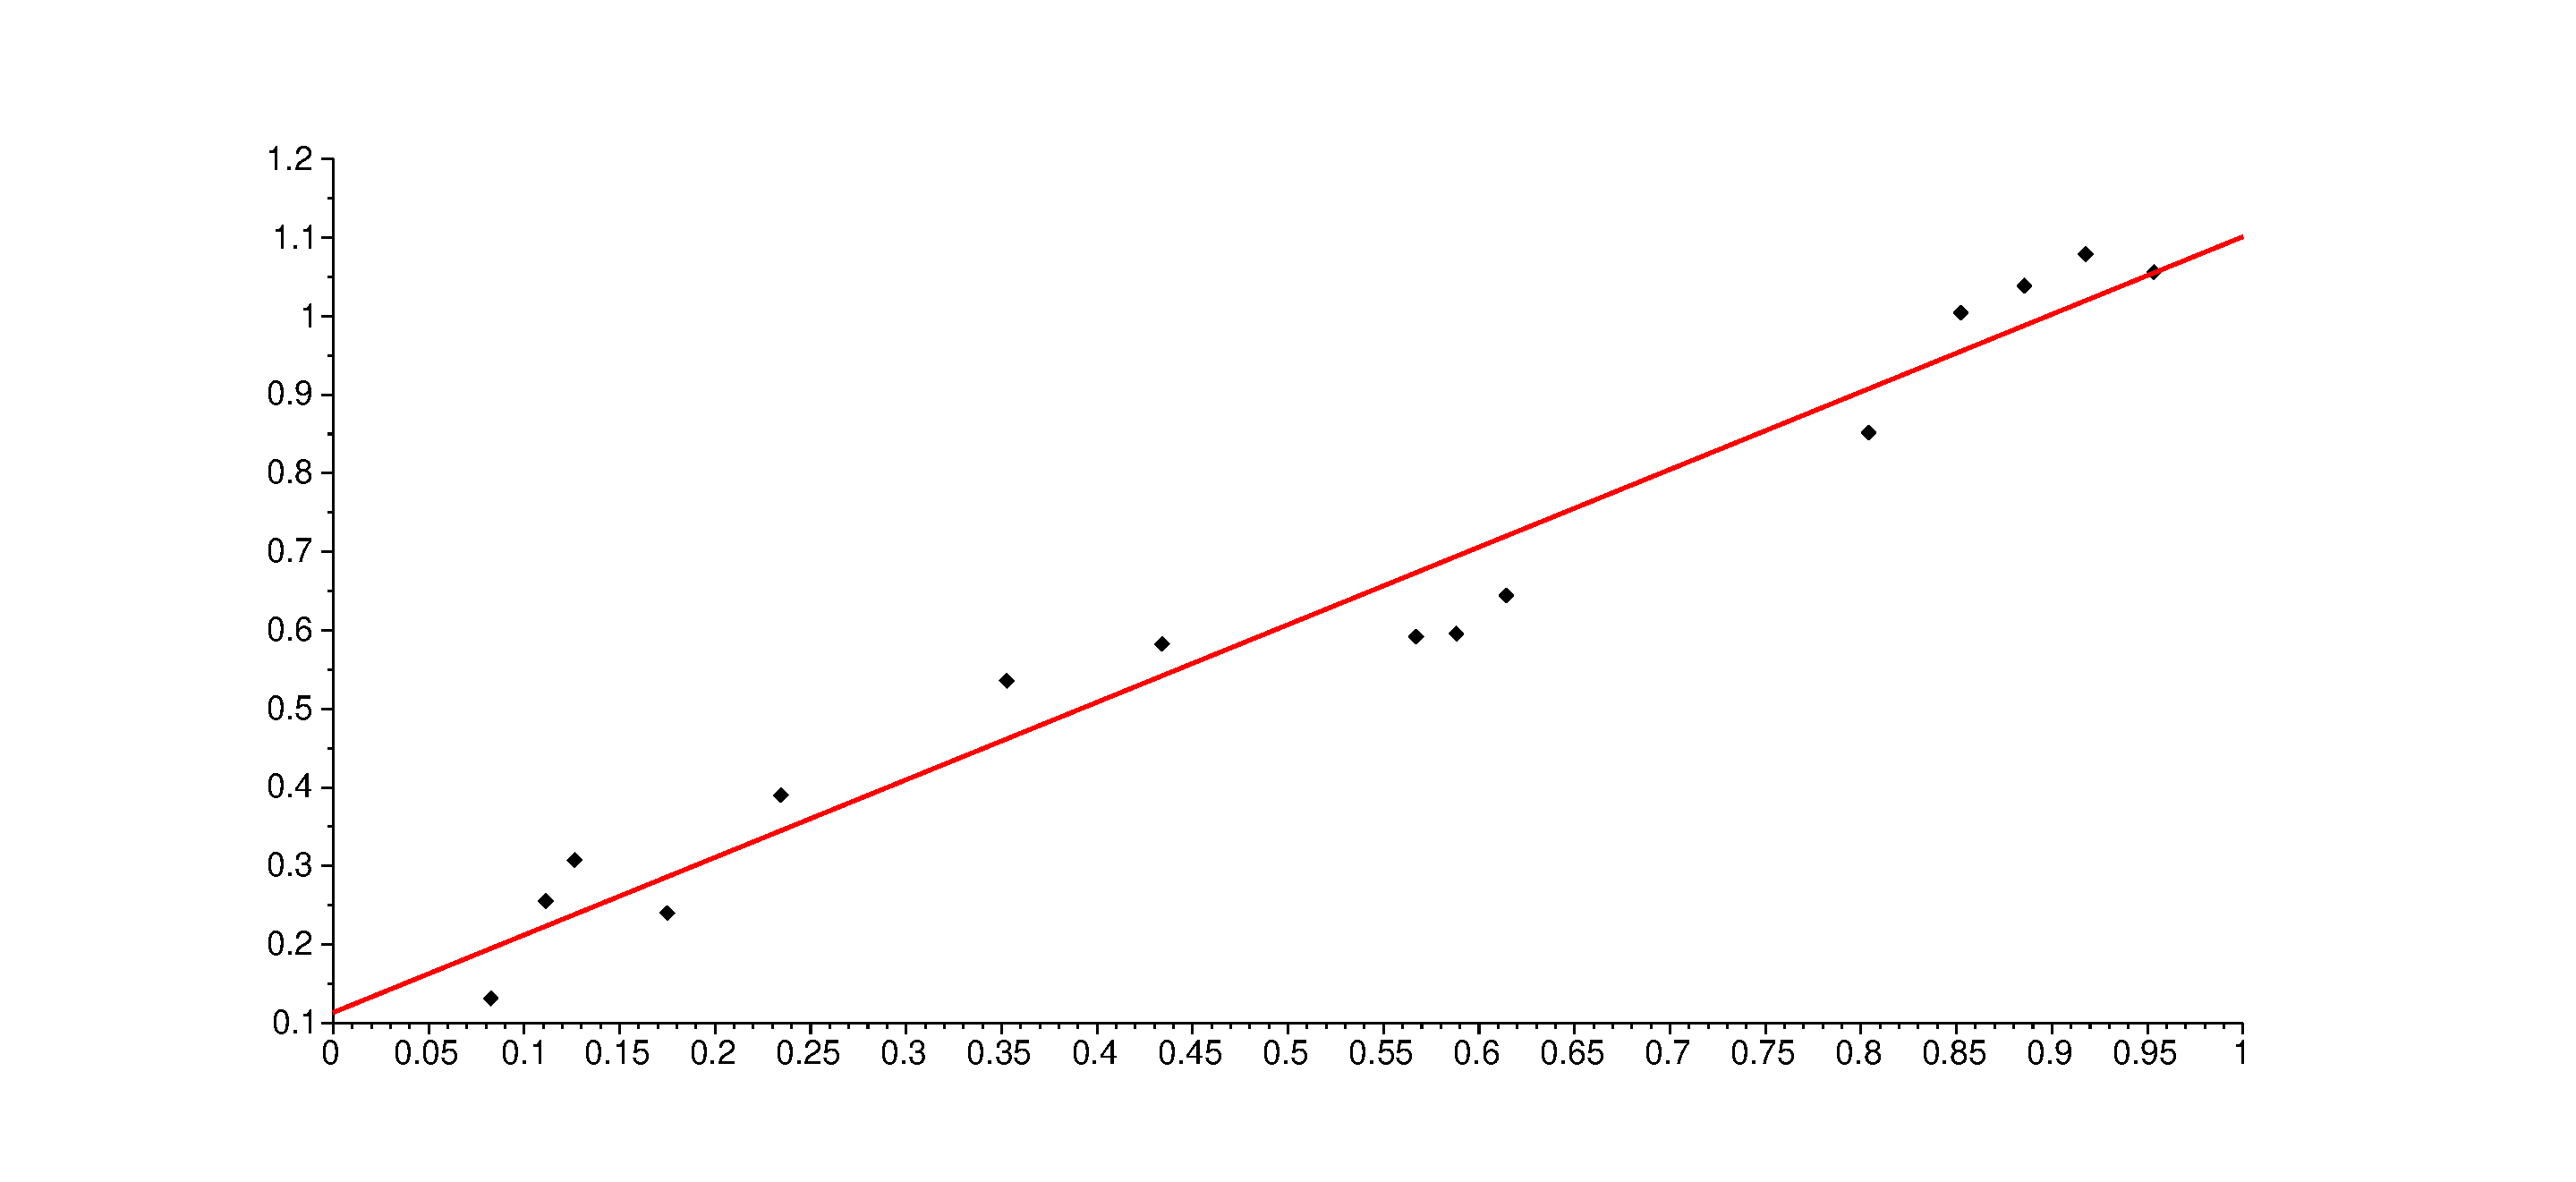
\includegraphics[width=15cm,angle=0]{./cap_aproxfun/pics/ajuste_reta.eps}
\caption{A reta que melhor se ajusta aos 15 pontos dados utilizando o critério dos mínimos quadrados.}
\label{minquad}
\end{center}
\end{figure}

Geralmente o critério mais usado consiste em minimizar a soma do quadrado das distâncias entre a coordenadas $y_j$ e a função desejada em $f(x_j)$. Ou seja, encontre a  função $f(x)$ tal que 
\begin{eqnarray*}
  R &=&(f(x_1)-y_1)^2+(f(x_2)-y_2)^2+\cdots +(f(x_N)-y_N)^2\\
    &=&\sum_{j=1}^N (f(x_j)-y_j)^2
\end{eqnarray*}
seja o menor possível, que fornece o nome do método como \emph{método dos mínimos quadrados}.  Note que o \emph{resíduo} em $x_j$ é definido como $r_j=|f(x_j)-y_j|$. 




\subsection{O problema linear}

Dado um conjunto de $N$ pontos, desejamos encontrar a \textit{reta} que melhor se ajusta a esses pontos de tal forma a minimizar o resíduo.

Ou seja, encontre a curva $f(x)=a_1+a_2 x$ tal que 
\begin{eqnarray*}
  R(a_1,a_2) &=\sum_{j=1}^N (f(x_j)-y_j)^2 = \sum_{j=1}^N (a_1 + a_2 x_j-y_j)^2
\end{eqnarray*}
seja o menor possível.

O objetivo é encontrar $a_1, a_2$ e geralmente temos muito mais equações do que incógnitas, i.e.,
\begin{eqnarray*}
 a_1+a_2 x_1 &=&y_1 \\
 a_1+a_2 x_2 &=&y_2 \\
 a_1+a_2 x_3 &=&y_3 \\
  \vdots     &=& \vdots \\
 a_N+a_2 x_N &=&y_N   
\end{eqnarray*}
ou simplesmente $V\vec a= \vec y$.

O mínimo de $R$ ocorre quando quando a derivada primeira é igual a zero:
\begin{eqnarray*}
  \frac{\partial R}{\partial a_1} &=& \frac{\partial }{\partial a_1} \sum_{j=1}^N (a_1 + a_2 x_j-y_j)^2 =0 \\
  \frac{\partial R}{\partial a_2} &=& \frac{\partial }{\partial a_2} \sum_{j=1}^N (a_1 + a_2 x_j-y_j)^2 =0 
\end{eqnarray*}
ou seja,
\begin{eqnarray*}
   2 \sum_{j=1}^N (a_1 + a_2 x_j-y_j)\cdot 1 &=&0 \\
   2 \sum_{j=1}^N (a_1 + a_2 x_j-y_j)\cdot x_j &=&0 
\end{eqnarray*}
e isolando as incógnitas temos
\begin{eqnarray*}
   a_1\sum_{j=1}^N 1 + a_2 \sum_{j=1}^Nx_j &=&\sum_{j=1}^N y_j\\
   a_1\sum_{j=1}^N x_j + a_2 \sum_{j=1}^Nx_j^2 &=&\sum_{j=1}^N y_jx_j
\end{eqnarray*}

Na forma matricial obtemos
\begin{equation}
  \begin{bmatrix}
     \sum_{j=1}^N 1 &  \sum_{j=1}^N x_j \\
     \sum_{j=1}^N x_j &  \sum_{j=1}^N x_j^2 
  \end{bmatrix}
  \begin{bmatrix}
     a_1 \\
     a_2 
  \end{bmatrix}=
  \begin{bmatrix}
     \sum_{j=1}^N y_j \\
     \sum_{j=1}^N x_j y_j 
  \end{bmatrix}
\end{equation}

Observe que é equivalente ao problema matricial
\begin{equation}
   Ma := V^TV a = V^Ty
\end{equation}


% Considere o sistema linear dado por
% $Ax=b$
% onde $A$ é uma matriz $n\times m$ e $b$ é um vetor de $n$ linhas. Assumimos as seguintes hipóteses:
% \begin{itemize}
% \item $n\geq m$. O número de linhas é igual ou superior ao número de colunas. (Mais equações que incógnitas)
% \item O posto de $A$ é $m$, i.e., existem $m$ linhas L.I. Isso implica que $Av=0$ apenas quando $v=0$
% \end{itemize}

% Neste caso, não seremos necessariamente capazes de encontrar um vetor $x$ que satisfaça exatamente a equação $Ax=b$, pelo que estamos interessamos no problema de encontrar o vetor $x$ (ordem m) que minimiza o erro quadrático dado por:
% \begin{equation}\label{defEm}
% E:=\sum_{j=1}^N \left[z_i- b_i\right]^2
% \end{equation}
% onde $z=Ax$ e $z_i$ é linha $i$ do vetor $z$, dado por:
% \begin{equation}\label{Axi}
% z_j=(Ax)_j=\sum_{j=1}^m a_{ij} x_j,\quad j=1,\cdots,n
% \end{equation}
% onde $a_{ij}$ é o elemento de $A$ na linha $i$ e coluna $j$.
% Substituindo (\ref{Axi}) em (\ref{defEm})
% \begin{equation}\label{erro}
% E:=\sum_{j=1}^N \left[\sum_{j=1}^m a_{ij} x_j- b_i\right]^2
% \end{equation}
% Esta é uma função diferenciável nos coeficientes $x_j$ e portanto todo ponto de mínimo acontece quando $\nabla E=0$, ou seja, quando $$\frac{\partial}{\partial x_l}E=0,\forall 1\leq l \leq m $$

% O que implica a seguinte condição
% \begin{eqnarray*}
% 0=\frac{\partial}{\partial x_l}E=\sum_{j=1}^N 2\left[\sum_{j=1}^m a_{ij} x_j- b_i\right] a_{il}, ~~~l=1,\cdots, m
% \end{eqnarray*}
% Equivalente a
% \begin{eqnarray*}
% \sum_{j=1}^N\sum_{j=1}^m  a_{il}x_j a_{ij}=\sum_{j=1}^Na_{il}b_i,~~~l=1,\cdots, m
% \end{eqnarray*}
% que pode ser reescrito na forma vetorial como:
% \begin{eqnarray}\label{cond_vet}
% \left[
% \begin{array}{c}
% \sum_{j=1}^N\sum_{j=1}^m   a_{i1}x_ja_{ij}\\
% \sum_{j=1}^N\sum_{j=1}^m   a_{i2}x_ja_{ij}\\
% \vdots\\
% \sum_{j=1}^N\sum_{j=1}^m   a_{im}x_ja_{ij}\\
% \end{array}
% \right]
% =
% \left[
% \begin{array}{c}
% \sum_{j=1}^Na_{i1}b_i\\
% \sum_{j=1}^Na_{i2}b_i\\
% \vdots\\
% \sum_{j=1}^Na_{im}b_i
% \end{array}
% \right]
% \end{eqnarray}
% Observamos agora que a expressão (\ref{cond_vet}) é equivalente ao seguinte problema matricial:
% 
% \begin{equation}\framebox[100 pt][c]{$A^TA x = A^Tb$}\end{equation}

\begin{teo}
A matriz $M=V^TV$ é quadrada de ordem $2$ e é inversível sempre que o posto da matriz $V$ é igual a número de colunas $m$.
\end{teo}
\begin{proof}
Para provar que $M$ é invertível precisamos mostrar que $Mv=0$ implica $v=0$:
$$Mv=0\Longrightarrow V^TVv=0$$
tomando o produto interno da expressão $0=V^TVv$ com $v$, temos:
$$0=\left<V^TVv,v\right>=\left<Vv,Vv\right>=\|Vv\|^2$$
Então se $Mv=0$, $Vv=0$, como o posto de $V$ é igual ao número de colunas, $v=0$.
\end{proof}
\begin{lem}
 A matrix $M=V^TV$ é simétrica.
\end{lem}
\begin{proof}
Isso é facilmente provado pelo seguinte argumento:
$$M^T=(V^TV)^T=(V)^T(V^T)^T=V^TV=M$$
\end{proof}




\begin{ex} Encontre a função do tipo $f(x)=ax$ que melhor se aproxima dos seguintes pontos:
  \begin{equation*}
    (0,-0,1), (1,~2), (2,~3,7) ~ \hbox{e} ~(3,~7).  
  \end{equation*}
\end{ex}
\begin{sol}
Defina $$E_q=[f(x_1)-y_1]^2+[f(x_2)-y_2]^2+[f(x_3)-y_3]^2+[f(x_4)-y_4]^2$$
temos que
\begin{eqnarray*}
E_q&=&[f(0)+0,1]^2+[f(1)-2]^2+[f(2)-3,7]^2+[f(3)-7]^2\\
&=&[0,1]^2+[a-2]^2+[2a-3,7]^2+[3a-7]^2
\end{eqnarray*}

Devemos encontrar o parâmetro $a$ que minimiza o erro, portanto, calculamos:
\begin{eqnarray*}
\frac{\partial E_q}{\partial a}&=&2[a-2]+4[2a-3,7]+6[3a-7]=28a-60,8
\end{eqnarray*}
Portanto o valor de $a$ que minimiza o erro é $a=\frac{60,8}{28}$.
\ifisscilab
\begin{verbatim}
x=[0 1 2 3]'
y=[-.1 2 3.7 7]'
plot2d(x,y,style=-4)
\end{verbatim}
\fi
\end{sol}

\begin{ex}Encontre a função do tipo $f(x)=bx+a$ que melhor aproxima os pontos:
  \begin{equation*}
    (0,-0,1), (1,~2), (2,~3,7) ~ \hbox{e} ~(3,~7).  
  \end{equation*}
\end{ex}
\begin{sol}
\begin{eqnarray*}
E_q&=&[f(0)+0,1]^2+[f(1)-2]^2+[f(2)-3,7]^2+[f(3)-7]^2\\
&=&[a+0,1]^2+[a+b-2]^2+[a+2b-3,7]^2+[a+3b-7]^2
\end{eqnarray*}

Devemos encontrar os parâmetros $a$ $b$ que minimizam o erro, por isso, calculamos as derivadas parciais:
\begin{eqnarray*}
\frac{\partial E_q}{\partial a}&=&2[a+0,1]+2[a+b-2]+2[a+2b-3,7]+2[a+3b-7]\\
\frac{\partial E_q}{\partial b}&=&2[a+b-2]+4[a+2b-3,7]+6[a+3b-7]
\end{eqnarray*}



O erro mínimo acontece quando as derivadas são nulas, ou seja:
\begin{eqnarray*}
8a+12b&=&25,2\\
12a+28b&=&60,8
\end{eqnarray*}
Cuja solução é dada por $a=-0,3$ e $b=2,3$.
Portanto a função que procuramos é $f(x)=-0,3 +2,3x$.  
\end{sol}


\subsection{Ajuste polinomial}

Dado um conjunto de $n$ pontos, desejamos encontrar o \textit{polinômio} de grau $p$ que melhor se ajusta a esses pontos de tal forma a minimizar o resíduo, ou seja, encontrar a curva $f(x)=a_1+a_2 x+...+a_{p+1}x^{p}$ tal que 
\begin{eqnarray*}
  R(a_1,...,a_{p+1}) &=&\sum_{j=1}^N (f(x_j)-y_j)^2 \\
                 &=&\sum_{j=1}^N (a_1 + a_2 x_j+...+a_{p+1}x_j^p-y_j)^2
\end{eqnarray*}
seja o menor possível.

O objetivo é encontrar as incógnitas $a_i$ que minimizam a soma do quadrado do resíduo.

O mínimo de $R$ encontra-se quando a derivada primeira é igual a zero:
\begin{eqnarray*}
  \frac{\partial R}{\partial a_1}     &=& \frac{\partial }{\partial a_1}     \sum_{j=1}^n (a_1 + a_2 x_j+...+a_{p+1}x_j^p-y_j)^2 =0 \\
  \vdots &=& \vdots \\
  \frac{\partial R}{\partial a_{p+1}} &=& \frac{\partial }{\partial a_{p+1}} \sum_{j=1}^n (a_1 + a_2 x_j+...+a_{p+1}x_j^p-y_j)^2 =0 
\end{eqnarray*}
ou seja,
\begin{eqnarray*}
   2 \sum_{j=1}^n (a_1 + a_2 x_j+...+a_{p+1}x_j^p-y_j)\cdot 1    &=&0 \\
  \vdots &=& \vdots \\
   2 \sum_{j=1}^n (a_1 + a_2 x_j+...+a_{p+1}x_j^p-y_j)\cdot x_j^p&=&0 
\end{eqnarray*}
e isolando as incógnitas temos
\begin{eqnarray*}
   a_1\sum_{j=1}^n 1     + a_2 \sum_{j=1}^Nx_j      +...+a_{p+1} \sum_{j=1}^Nx_j^{p} &=\sum_{j=1}^N y_j\\
  \vdots &= \vdots \\
   a_1\sum_{j=1}^n x_j^p + a_2 \sum_{j=1}^Nx_j^{p+1}+...+a_{p+1} \sum_{j=1}^Nx_j^{2p} &=\sum_{j=1}^N y_jx_j^{p}
\end{eqnarray*}

Na forma matricial obtemos
\begin{equation}
  \begin{bmatrix}
     \sum 1     &  \sum  x_j   & \cdots & \sum x_j^p\\
     \sum x_j   &  \sum  x_j^2 &        & \sum x_j^{p+1}\\
     \vdots     &              & \ddots & \vdots    \\
     \sum x_j^p &  \sum  x_j^{p+1} & \cdots & \sum x_j^{2p}
  \end{bmatrix}
  \begin{bmatrix}
     a_1 \\
     a_2 \\
     \vdots \\
     a_{p+1}
  \end{bmatrix}=
  \begin{bmatrix}
     \sum y_j \\
     \sum x_j y_j \\
     \vdots \\
     \sum x_j^p y_j 
  \end{bmatrix}
\end{equation}

Na forma matricial temos 
\begin{equation}
   Ma := V^TV a = V^Ty
\end{equation}




\subsection{Ajuste linear de curvas}
Seja $f_1(x), f_2(x),\ldots, f_m(x)$ um conjunto de $m$ funções e $(x_i,y_i)$ um conjunto de $n$ pontos. Procuram-se os coeficientes $a_1,a_2,\ldots, a_m$ tais que a função dada por
$$f(x)=a_1f_1(x)+a_2f_2(x)+\ldots+a_mf_m(x)$$
minimiza o resíduo dado por
$$R= \sum_{j=1}^n \left[f(x_i)-y_i\right]^2$$
como $f(x)=\sum_{j=1}^m a_jf_j(x)$, temos
$$R= \sum_{j=1}^n \left[\sum_{j=1}^m a_jf_j(x_i)-y_i\right]^2$$

Este problema é equivalente a resolver pelo métodos dos mínimos quadrados o seguinte sistema linear:
$$
\left[
\begin{array}{cccc}
f_1(x_1)&f_2(x_1) & \cdots & f_m(x_1)\\
f_1(x_2)&f_2(x_2) & \cdots & f_m(x_2)\\
f_1(x_3)&f_2(x_3) & \cdots & f_m(x_3)\\
\vdots & \vdots & \ddots & \vdots\\
f_1(x_n)&f_2(x_n) & \cdots & f_m(x_n)
\end{array}
\right]
\left[
\begin{array}{c}
a_1\\
a_2\\
\vdots\\
a_m
\end{array}
\right]=\left[\begin{array}{c}
y_1\\
y_2\\
y_3\\
\vdots\\
y_n
\end{array}
\right]
$$



\begin{ex} Encontre a reta que melhor aproxima o seguinte conjunto de dados:
  \begin{center}
    \begin{tabular}{|c|c|}
      \hline
      $x_i$ & $y_i$\\
      \hline
      $0,01$ & $1,99$\\
      $1,02$ & $4,55$\\
      $2,04$ & $7,20$\\
      $2,95$ & $9,51$\\
      $3,55$ & $10,82$\\
      \hline
    \end{tabular}
  \end{center}
\end{ex}
\begin{sol}
Desejamos encontrar os valores de $a$ e $b$ tais que a função $f(x)=ax+b$ melhor se ajusta aos pontos da tabela. Afim de usar  o critério dos mínimos quadrados, escrevemos o problema na forma matricial dada por:
$$
\left[\begin{array}{cc}
0,01 &1\\
1,02 &1\\
2,04 &1\\
2,95 &1\\
3,55 &1
\end{array}
\right]
\left[\begin{array}{c}
a\\
b
\end{array}
\right]
=
\left[\begin{array}{c}
1,99\\
4,55\\
7,2\\
9,51\\
10,82
\end{array}
\right]
$$

Multiplicamos agora ambos os lados pela transposta:
\begin{equation*}
  \begin{bmatrix}
    0,01 &1,02 &2,04 &2,95 &3,55\\
    1 &1 &1 &1 &1
    \end{bmatrix}
\end{equation*}
o que fornece:
\begin{eqnarray*}
  \left[\begin{array}{ccccc}
      0,01 &1,02 &2,04 &2,95 &3,55\\
      1 &1 &1 &1 &1
    \end{array}
  \right]
  \left[\begin{array}{cc}
      0,01 &1\\
      1,02 &1\\
      2,04 &1\\
      2,95 &1\\
      3,55 &1
    \end{array}
  \right]
  \left[\begin{array}{c}
      a\\
      b
    \end{array}
  \right]
  &=&\\
  &\left[\begin{array}{ccccc}
      0,01 &1,02 &2,04 &2,95 &3,55\\
      1 &1 &1 &1 &1
    \end{array}
  \right]
  \left[\begin{array}{c}
      1,99\\
      4,55\\
      7,2\\
      9,51\\
      10,82
    \end{array}
  \right]  
\end{eqnarray*}
$$\left[
  \begin{array}{cc}
    26,5071  & 9,57 \\
    9,57  &     5
  \end{array}
\right]
\left[
  \begin{array}{c}
    a   \\
    b
  \end{array}
\right]=
\left[
  \begin{array}{c}
    85,8144  \\
    34,07
  \end{array}
\right]
$$

A solução desse sistema é $a=2,5157653$ e $b=1,9988251$

A tabela abaixo mostra os valores dados e os valores ajustados:
\begin{center}
\begin{tabular}{|c|c|c|c|}
\hline
$x_i$ & $y_i$& $ax_i+b$& $ax_i+b-y_i$\\
\hline
$0,01$ & $1,99$ & $2,0239828$ & $0,0339828$\\
$1,02$ & $4,55$ & $4,5649057$ & $0,0149057$ \\
$2,04$ & $7,2$ & $7,1309863$ & $-0,0690137$ \\
$2,95$ & $9,51$ & $9,4203327$ & $-0,0896673$  \\
$3,55$ & $10,82$ & $10,929792$ & $0,1097919$ \\
\hline
\end{tabular}  
\end{center}
\end{sol}

\subsection*{Exercícios}

\begin{Exercise}Encontrar  a parábola $y=ax^2+bx+c$ que melhor aproxima o seguinte conjunto de dados:
  \begin{center}
    \begin{tabular}{|c|c|}
      \hline
      $x_i$ & $y_i$\\
      \hline
      $0,01$ & $1,99$\\
      $1,02$ & $4,55$\\
      $2,04$ & $7,2$\\
      $2,95$ & $9,51$\\
      $3,55$ & $10,82$\\
      \hline
    \end{tabular}    
  \end{center}
  e complete a tabela:
  \begin{center}
    \begin{tabular}{|c|c|c|c|}
      \hline
      $x_i$ & $y_i$& $ax_i^2+bx_i+c$& $ax_i^2+bx_i+c-y_i$\\
      \hline
      $0,01$ & $1,99$& &\\
      $1,02$ & $4,55$&& \\
      $2,04$ & $7,20$&  & \\
      $2,95$ & $9,51$  &  & \\
      $3,55$ & $10,82$&&\\
      \hline
    \end{tabular}
  \end{center}
\end{Exercise}
\begin{Answer}
  \begin{tiny}
$y=-0,0407898x^2+ 2,6613293x+ 1,9364598$    
\begin{equation*}
\begin{tabular}{|c|c|c|c|}
\hline
$x_i$ & $y_i$& $ax_i^2+bx_i+c$& $ax_i^2+bx_i+c-y_i$\\
\hline
0,01 & 1,99&1,963069&-0,0269310  \\
1,02 & 4,55&4,6085779&    0,0585779  \\
2,04 & 7,2&7,1958206  &  -0,0041794  \\
2,95 & 9,51& 9,4324077   &-0,0775923   \\
3,55 & 10,82& 10,870125   &0,0501249\\
\hline
\end{tabular}  
\end{equation*}
  \end{tiny}
\end{Answer}


\begin{Exercise} Dado o seguinte conjunto de dados
  \begin{equation*}
    \begin{tabular}{|c|c|}
      \hline
      $x_i$ & $y_i$\\
      \hline
      0,0 &  31\\
      0,1 &  35\\
      0,2 &  37\\
      0,3 &  33\\
      0,4 &  28\\
      0,5 &  20\\
      0,6 &  16\\
      0,7 &  15\\
      0,8 &  18\\
      0,9 &  23\\
      1,0 &  31\\
      \hline
    \end{tabular}    
  \end{equation*}
\begin{itemize}
\item Encontre a função do tipo $f(x)=a+b\sin(2\pi x)+c\cos(2\pi x)$ que melhor aproxima os valores dados.
\item Encontre a função do tipo $f(x)=a+bx+cx^2+dx^3$ que melhor aproxima os valores dados.
\end{itemize}
\end{Exercise}
\begin{Answer}
  \begin{tiny}
      $a=25,638625$, $b=9,8591874$, $c=4,9751219$ e   $a=31,475524$, $b=65,691531$, $c=-272,84382$, $d=208,23621$.
  \end{tiny}
\end{Answer}

\section{Aproximando problemas não lineares por problemas lineares}

Eventualmente, problemas de ajuste de curvas podem recair num sistema não linear. Por exemplo, para ajustar função $y=Ae^{bx}$ ao conjunto de pontos $(x_1,y_1)$, $(x_2,y_2)$ e $(x_3,y_3)$, temos que minimizar o resíduo\footnote{A soma do quadrado dos resíduos.} 
$$
R=(Ae^{x_1b}-y_1)^2+(Ae^{x_2b}-y_2)^2+(Ae^{x_3b}-y_3)^2
$$
ou seja, resolver o sistema
\begin{eqnarray*}
\frac{\partial R}{\partial A} &=& 2(Ae^{x_1b}-y_1)e^{x_1b}+2(Ae^{x_2b}-y_2)e^{x_2b}+2(Ae^{x_3b}-y_3)e^{x_3b}=0\\
\frac{\partial R}{\partial b} &=& 2Ax_1(Ae^{x_1b}-y_1)e^{x_1b} + 2Ax_2(Ae^{x_2b}-y_2)e^{x_2b} \\
&+& 2Ax_3(Ae^{x_3b}-y_3)e^{x_3b}=0
\end{eqnarray*}
que é não linear em $A$ e $b$. Esse sistema pode ser resolvido pelo método de Newton-Raphson, o que pode se tornar custoso, ou mesmo inviável quando não dispomos de uma boa aproximação da solução para inicializar o método.

Felizmente, algumas famílias de curvas admitem uma transformação que nos leva a um problema linear. No caso da curva $y=Ae^{bx}$, observe que $\ln y=\ln A+bx$. Assim, em vez de ajustar a curva original $y=Ae^{bx}$ a tabela de pontos, ajustamos a curva submetida a transformação logarítmica
$$
\tilde y:=a_1+a_2 \tilde x=\ln A+bx.
$$
Usamos os pontos $(\tilde x_j,\tilde y_j):=(x_j,\ln y_j)$, $j=1,2,3$ e resolvemos o sistema linear
$$
V^T V \left[\begin{array}{c} a_1\\a_2 \end{array}\right]=V^T\left[\begin{array}{c}\tilde{y}_1\\\tilde{y}_2\\\tilde{y}_3 \end{array}\right],
$$
onde
$$
A=\left[\begin{array}{cc} 1&x_1\\1&x_2\\1&x_3 \end{array}\right]
$$
\begin{ex}Encontre uma curva da forma $y=Ae^x$ que melhor ajusta os pontos $(1, 2)$, $(2, 3)$ e $(3, 5)$.
\end{ex}
Temos
$$
A=\left[\begin{array}{cc} 1&1\\1&2\\1&3 \end{array}\right]
$$
e a solução do sistema leva em $B=0,217442$ e $b=0,458145$. Portanto, $A=e^{0,217442}=1,24289$.

\begin{obs}
Os coeficientes obtidos a partir dessa linearização são aproximados, ou seja, são diferentes daqueles obtidos quando aplicamos mínimos quadrados não linear. Observe que estamos minimizando $\displaystyle\sum_i [\ln y_i -\ln (f(x_i))]^2$ em vez de $\displaystyle\sum_i [ y_i -f(x_i)]^2$. No exemplo resolvido, a solução do sistema não linear original seria $A=1,19789$ e $B=0,474348$
\end{obs}

\begin{obs}
Mesmo quando se deseja resolver o sistema não linear, a solução do problema linearizado pode ser usada para construir condições iniciais.
\end{obs}


A próxima tabela apresenta algumas curvas e transformações que linearizam o problema de ajuste.
$$
\begin{array}{|c|c|c|}   \hline
\hbox{curva}    &\hbox{transformação}&\hbox{problema linearizado}\\ \hline
y=ae^{bx}       &\tilde y=\ln y       & \tilde y=\ln a+ bx\\ \hline
y=ax^b          &\tilde y=\ln y       & \tilde y=\ln a+ b\ln x\\ \hline
y=ax^be^{cx}    &\tilde y=\ln y       & \tilde y=\ln a+ b\ln x+cx\\ \hline
y=ae^{(b+cx)^2} &\tilde y=\ln y       & \tilde y=\ln a+b^2+ bc x+c^2x^2\\ \hline
y=\frac{a}{b+x} &\tilde y=\frac{1}{y} & \tilde y=\frac{b}{a}+\frac{1}{a}x\\ \hline
y=A\cos(\omega x+\phi)   & - &  y=a\cos(\omega x)-b\sin(\omega x) \\
\omega\ \hbox{conhecido} &   &  a=A\cos(\phi),\ b=A\sin(\phi) \\ \hline
\end{array}
$$

\begin{ex}
Encontre a função $f$ da forma $y=f(x)=A\cos(2 \pi x+\phi)$ que ajusta a tabela de pontos
$$
\begin{tabular}{|c|c|}
\hline
$x_i$ & $y_i$\\
\hline
0,0  &   9,12\\
0,1  &    1,42\\
0,2  &  - 7,76\\
0,3  &  - 11,13\\
0,4  &  - 11,6\\
0,5  &  - 6,44\\
0,6  &    1,41\\
0,7  &    11,01\\
0,8  &    14,73\\
0,9  &    13,22\\
1,0  &    9,93 \\
\hline
\end{tabular}
$$
\end{ex}
\begin{sol}
Usando o fato que $y=A\cos(2 \pi x+\phi)=a\cos(2 \pi x)-b\sin(2 \pi x)$, onde $a=A\cos(\phi)$ e $b=A\sin(\phi)$, $z=[\begin{array}{cc}a &b\end{array}]^T$ é solução do problema
$$
B^TBz=B^Ty,
$$
onde
$$
B\!=\!\left[\begin{array}{cc}\cos(2 \pi x_0)& -\sin(2 \pi x_0)\\ \cos(2 \pi x_1)& -\sin(2 \pi x_1)\\ \vdots\\ \cos(2 \pi x_{10})& -\sin(2\pi x_{10}) \end{array}\right]\!=\!\left[\begin{array}{cc}  1.     &      0.\\
    0,8090170 & - 0,5877853\\
    0,3090170 & - 0,9510565\\
  - 0,3090170 & - 0,9510565\\
  - 0,8090170 & - 0,5877853\\
  - 1,0000000 &   0,0000000\\
  - 0,8090170 &   0,5877853\\
  - 0,3090170 &   0,9510565\\
    0,3090170 &   0,9510565\\
    0,8090170 &   0,5877853\\
    1,0000000 &   0,0000000   \end{array}\right].
$$
Assim, $a=7,9614704$ e $b=11,405721$ e obtemos o seguinte sistema:
$$
\left\{\begin{array}{c}
A\cos(\phi)=7,9614704\\ A\sin(\phi)=11,405721
\end{array}\right..
$$
Observe que
$$
A^2=7,9614704^2+11,405721^2
$$
e, escolhendo $A>0$, $A=13,909546$ e
$$
\sin(\phi)=\frac{11,405721}{13,909546}=0,8199923
$$
Assim, como $\cos\phi$ também é positivo, $\phi$ é um ângulo do primeiro quadrante:
$$
\phi=0,9613976
$$
Portanto $f(x)=13,909546\cos(2\pi x+0,9613976)$. Observe que nesse exemplo a solução do problema linear é a mesma do problema não linear.  
\end{sol}

\begin{ex}
Encontre a função $f$ da forma $y=f(x)=\frac{a}{b+x}$ que ajusta a tabela de pontos
$$
\begin{tabular}{|c|c|}
\hline
$x_i$ & $y_i$\\
\hline
0,0  & 101\\
0,2  &  85\\
0,4  &  75\\
0,6  &  66\\
0,8  &  60\\
1,0  &  55 \\
\hline
\end{tabular}
$$
usando uma das transformações tabeladas.
\end{ex}
\begin{sol}
Usando o fato que $Y=\frac{1}{y}=\frac{b}{a}+\frac{1}{a}x$, $z=[\begin{array}{cc}\frac{b}{a} &\frac{1}{a}\end{array}]^T$ é solução do problema
$$
A^TAz=A^TY,
$$
onde
$$
A=\left[\begin{array}{cc}1& x_1\\ 1& x_2\\ 1&x_3\\1&x_4 \\ 1&x_5 \\ 1&x_6 \end{array}\right]=\left[\begin{array}{cc}
  1 &  0,0\\
  1 &  0,2\\
  1 &  0,4\\
  1 &  0,6\\
  1 &  0,8\\
  1 &  1,0
\end{array}\right]
$$
e
$$
Y=\left[\begin{array}{c}
  1/y_1\\
    1/y_2\\
    1/y_3\\
    1/y_4\\
    1/y_5\\
    1/y_6
\end{array}\right]=\left[\begin{array}{c}
  0,0099010\\
  0,0117647\\
  0,0133333\\
  0,0151515\\
  0,0166667\\
  0,0181818
\end{array}\right]
$$
Assim, $\frac{1}{a}=0,0082755$ e $\frac{b}{a}=0,0100288$ e, então, $a=120,83924$ e $b=1,2118696$, ou seja, $f(x)=\frac{120,83924}{1,2118696+x}$.  
\end{sol}


\section{Interpolação linear segmentada}\index{interpolação!linear segmentada}
Considere o conjunto $\left(x_i,y_i\right)_{j=1}^n$ de $n$ pontos. Assumiremos que $x_{i+1}>x_i$, ou seja, as abscissas são distintas e estão em ordem crescente. A função linear que interpola os pontos $x_i$ e $x_{i+1}$ no intervalo $i$ é dada por
$$P_i(x)=y_i \frac{(x_{i+1}-x)}{(x_{i+1}-x_i)} + y_{i+1} \frac{(x-x_i)}{(x_{i+1}-x_i)}$$

O resultado da interpolação linear segmentada é a seguinte função contínua definida por partes no intervalo $[x_1,x_n]$:
$$f(x)=P_i(x), ~~~~ x\in [x_i,x_{i+1}]$$

\begin{ex}
  Construa uma função linear por partes que interpola os pontos $(0,0)$, $(1,4)$, $(2,3)$, $(3,0)$, $(4,2)$, $(5,0)$.

A função procurada pode ser construída da seguinte forma:
\begin{equation*}
  f(x) = \left\{
    \begin{array}{ll}
      0\frac{x-1}{0-1} + 1\frac{x-0}{1-0} &, 0 \leq x < 1\\
      4\frac{x-2}{1-2} + 3\frac{x-1}{2-1} &, 1\leq x < 2\\
      3\frac{x-3}{2-3} + 0\frac{x-2}{3-2} &, 2\leq x \leq 3
    \end{array}
\right.
\end{equation*}
Simplificando, obtemos:
\begin{equation*}
  f(x) = \left\{
    \begin{array}{ll}
      x &, 0 \leq x < 1\\
      -x + 5 &, 1\leq x < 2\\
      -3x + 9 &, 2\leq x \leq 3
    \end{array}
\right.  
\end{equation*}
\end{ex}

A Figura \ref{fig:linear_segmentada} é um esboço da função $f(x)$ obtida. 
\ifisscilab
Ela foi gerada no \verb+Scilab+ usando os comandos:
\verbatiminput{./cap_aproxfun/codes/interpolacao_linear_segmentada/ex_linear_segmentada.sce}
\fi

\begin{figure}[htp]
\begin{center}
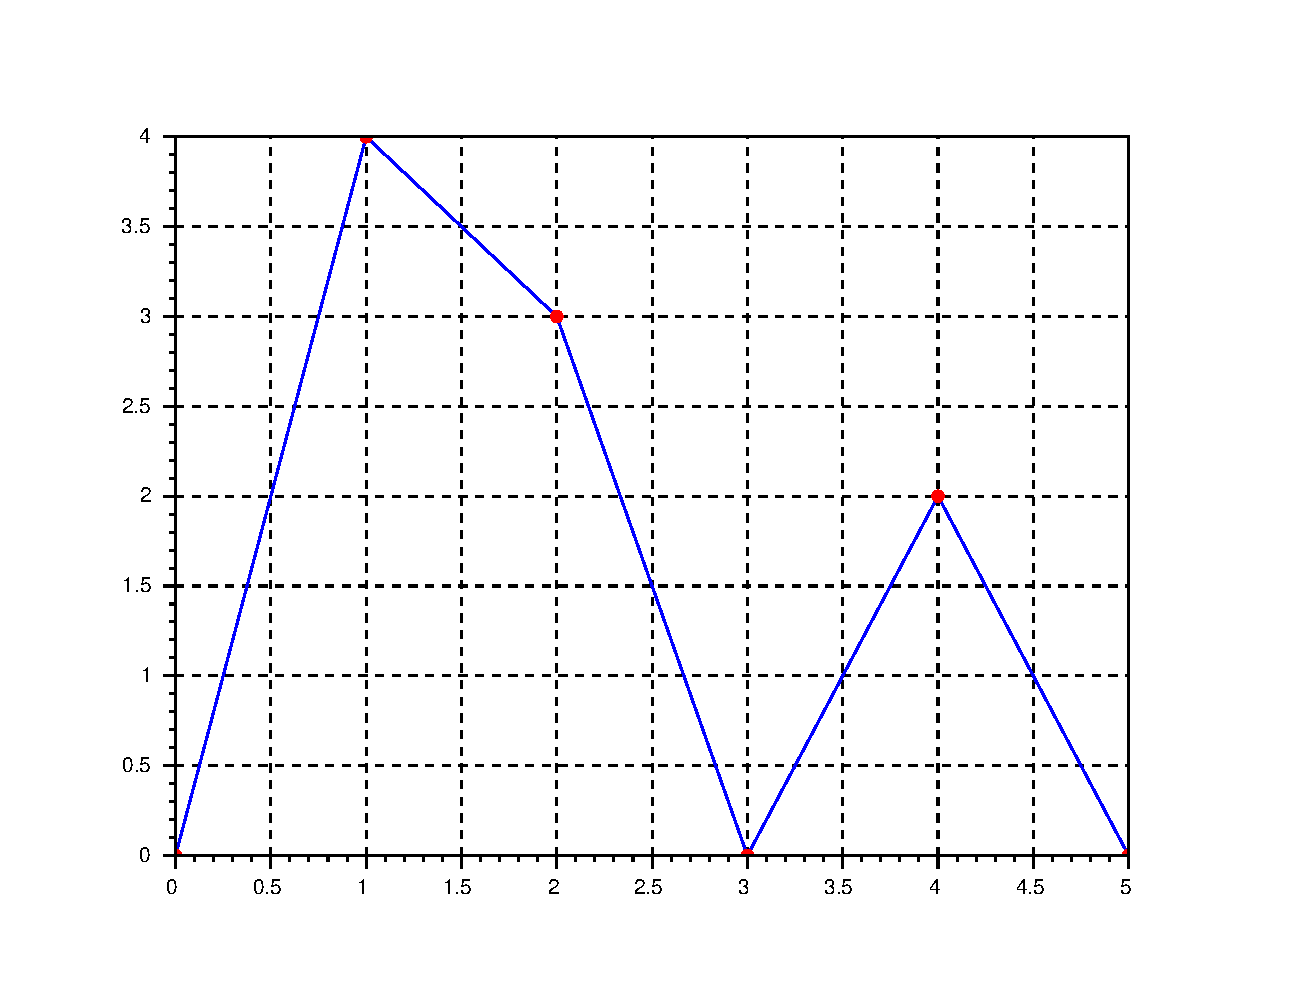
\includegraphics[scale=0.5]{./cap_aproxfun/pics/interpolacao_linear_segmentada.eps}
\caption{Interpolação linear segmentada.}
\label{fig:linear_segmentada}
\end{center}
\end{figure}


\section{Interpolação cúbica segmentada - spline}\index{interpolação!cúbica segmentada}\index{spline}
Dado um conjunto de $n$ pontos $\left(x_j,y_j\right)_{j=1}^n$ tais que $x_{j+1}>x_j$, ou seja, as abscissas são distintas e estão em ordem crescente; um spline cúbico que interpola estes pontos é uma função $s(x)$ com as seguintes propriedades:
\begin{itemize}
\item[i] Em cada segmento $[x_j,x_{j+1}]$, $j=1,2,\ldots n-1$ $s(x)$ é um polinômio cúbico.
\item[ii] para cada ponto, $s(x_j)=y_j$, i.e., o spline interpola os pontos dados.
\item[iii] $s(x)\in C^2$, i.e., é função duas vezes continuamente diferenciável.
\end{itemize}

Da primeira hipótese, escrevemos
$$s(x)=s_j(x),x \in [x_j,x_{j+1}],~~ j=1,\ldots, n-1$$
com
$$s_j(x)=a_j+b_j(x-x_j)+c_j(x-x_j)^2+d_j(x-x_j)^3$$
O problema agora consiste em obter os 4 coeficientes de cada um desses $n-1$ polinômios cúbicos.

Veremos que a simples definição de spline produz $4n-6$ equações linearmente independentes:
\begin{equation*}
\begin{array}{rcll}
s_j(x_j)&=&y_j,~~ &j=1,\ldots, n-1\\
s_{j}(x_{j+1})&=&y_{j+1},~~ &j=1,\ldots, n-1\\
s_{j}'(x_{j+1})&=&s_{j+1}'(x_{j+1}),~~ &j=1,\ldots, n-2\\
s_{j}''(x_{j+1})&=&s_{j+1}''(x_{j+1}),~~ &j=1,\ldots, n-2
\end{array}
\end{equation*}
Como
\begin{equation}\label{eq_1derivada}
s'_j(x)=b_j+2c_j(x-x_j)+3d_j(x-x_j)^2
\end{equation}
e
\begin{equation}\label{eq_2derivada}
s''_j(x)=2c_j+6d_j(x-x_j),
\end{equation}
temos, para $j=1,\ldots, n-1$, as seguintes equações
\begin{equation*}
\begin{array}{rcl}
a_j&=&y_j,\\
a_j+b_j(x_{j+1}-x_j)+c_j(x_{j+1}-x_j)^2+d_j(x_{j+1}-x_j)^3&=&y_{j+1},\\
b_j+2c_j(x_{j+1}-x_j)+3d_j(x_{j+1}-x_j)^2&=&b_{j+1},\\
c_j+3d_j(x_{j+1}-x_j)&=&c_{j+1},
\end{array}
\end{equation*}
Por simplicidade, definimos
$$
h_j=x_{j+1}-x_j
$$
e temos
\begin{equation}
\begin{array}{rcl}
a_j&=&y_j,\\
a_j+b_jh_j+c_jh_j^2+d_jh_j^3&=&y_{j+1},\\
b_j+2c_jh_j+3d_jh_j^2&=&b_{j+1},\label{eq3}\\
c_j+3d_jh_j&=&c_{j+1},
\end{array}
\end{equation}
que podem ser escrita da seguinte maneira
\begin{equation}\label{eq_an_spline}
a_j=y_j,
\end{equation}
\begin{equation}\label{eq_dn_spline}
d_j=\frac{c_{j+1}-c_j}{3h_j},
\end{equation}
\begin{equation}\label{eq_bn_spline}
  \begin{split}
    b_j &= \frac{y_{j+1}-y_j-c_jh_j^2-\frac{c_{j+1}-c_j}{3h_j}h_j^3}{h_j},\\
    &= \frac{3y_{j+1}-3y_j-3c_jh_j^2-c_{j+1}h_j^2+c_jh_j^2}{3h_j}\\
    &= \frac{3y_{j+1}-3y_j-2c_jh_j^2-c_{j+1}h_j^2}{3h_j}
  \end{split}
\end{equation}
Trocando o índice $j$ por $j-1$ na terceira equação \eqref{eq3}, $j=2,\ldots, n-1$
\begin{equation}
b_{j-1}+2c_{j-1}h_{j-1}+3d_{j-1}h_{j-1}^2=b_{j}  
\end{equation}
e, portanto,
\begin{equation}
  \begin{split}
    \frac{3y_{j}-3y_{j-1}-2c_{j-1}h_{j-1}^2-c_{j}h_{j-1}^2}{3h_{j-1}} &+ 2c_{j-1}h_{j-1}+c_{j}h_{j-1}-c_{j-1}h_{j-1} \\
    &=\frac{3y_{j+1}-3y_j-2c_jh_j^2-c_{j+1}h_j^2}{3h_j}.      
  \end{split}
\end{equation}
Fazendo as simplificações, obtemos:
\begin{equation}\label{eq_cn_spline}
  c_{j-1}h_{j-1}+c_j(2h_j+2h_{j-1})+c_{j+1}h_j=3\frac{y_{j+1}-y_j}{h_j}-3\frac{y_{j}-y_{j-1}}{h_{j-1}}.
\end{equation}
É costumeiro acrescentar a incógnita $c_n$ ao sistema. A incógnita $c_n$ não está relacionada a nenhum dos polinômios interpoladores. Ela é uma construção artificial que facilita o cálculo dos coeficientes do spline. Portanto, a equação acima pode ser resolvida para $j=2, \ldots, n-1$.

Para determinar unicamente os $n$ coeficientes $c_n$ precisamos acrescentar duas equações linearmente independentes às $n-2$ equações dadas por \eqref{eq_cn_spline}. Essas duas equações adicionais definem o tipo de spline usado.

\subsection{Spline natural}\index{spline!natural}

Uma forma de definir as duas equações adicionais para completar o sistema \eqref{eq_cn_spline} é impor condições de fronteira livres (ou naturais), ou seja,
\begin{equation}
S''(x_1)=S''(x_n)=0.
\end{equation}
Substituindo na equação \eqref{eq_2derivada}
$$
s''_1(x_1)=2c_1+6d_1(x_1-x_1)=0 \Longrightarrow c_1=0.
$$
e
$$
s''_{n-1}(x_n)=2c_{n-1}+6d_{n-1}(x_{n}-x_{n-1})=0 .
$$
Usando o fato que
$$
c_{n-1}+3d_{n-1}h_{n-1}=c_{n}
$$
temos que
$$
c_n=-3d_{n-1}(x_{n}-x_{n-1})+3d_{n-1}h_{n-1}=0.
$$
Essa duas equações para $c_1$ e $c_n$ juntamente com as equações \eqref{eq_cn_spline} formam um sistema de $n$ equações $Ac=z$, onde
\begin{equation}
A=\left[\begin{array}{ccccccc}
1 &0&0&0 &\cdots&0&0\\
h_1&2h_2+2h_{1}&h_2&0&\cdots&0&0\\
0&h_2&2h_3+2h_{2}&h_3&\cdots&0&0\\
\vdots&\vdots&\vdots&\vdots&\ddots&\vdots&\vdots\\
0&0&0&\cdots&h_{n-2} & 2h_{n-2}+2h_{n-1}&h_{n-1}\\
0&0&0&\cdots &0&0&1
\end{array}\right]  
\end{equation}
\begin{equation}
c = \left[\begin{array}{c}
c_1\\
c_2\\
\vdots\\
c_n
\end{array}\right]\qquad \hbox{e}\qquad
z = \left[\begin{array}{c}
0\\
3\frac{y_{3}-y_2}{h_2}-3\frac{y_{2}-y_{1}}{h_{1}}\\
3\frac{y_{4}-y_3}{h_3}-3\frac{y_{3}-y_{2}}{h_{2}}\\
\vdots\\
3\frac{y_{n-1}-y_{n-2}}{h_{n-2}}-3\frac{y_{n-2}-y_{n-3}}{h_{n-3}}\\
0
\end{array}\right]
\end{equation}
Observe que a matriz $A$ é diagonal dominante estrita e, portanto, o sistema $Ac=z$ possui solução única. Calculado $c$, os valores dos $a_n$, $b_n$ e $d_n$ são obtidos diretamente pelas expressões \eqref{eq_an_spline}, \eqref{eq_bn_spline} e \eqref{eq_dn_spline}, respectivamente.

\begin{ex}Construa um spline cúbico natural que passe pelos pontos $(2,~4,5)$, $(5,-1,9)$, $(9,~0,5)$ e $(12,-0,5)$.
\end{ex}
\begin{sol}
O spline desejado é uma função definida por partes da forma:
\begin{equation}
S(x)=\left\{\begin{array}{ll}
    a_1+b_1(x-2)+c_1(x-2)^2+d_1(x-2)^3 &, 2\leq x <5\\
    a_2+b_2(x-5)+c_2(x-5)^2+d_2(x-5)^3 &, 5\leq x <9\\
    a_3+b_3(x-9)+c_3(x-9)^2+d_3(x-9)^3 &, 9\leq x \leq 12
\end{array}\right..  
\end{equation}
Os coeficientes $c_1$, $c_2$ e $c_3$ resolvem o sistema $Ac = z$, onde
\begin{equation*}
A = \begin{bmatrix}
  1 &0&0&0 \\
  3&2\cdot 3+2\cdot 4&4&0\\
  0&4&2\cdot 4+2\cdot 3&3\\
  0&0&0&1
\end{bmatrix} = \begin{bmatrix}
  1 &0&0&0 \\
  3&14&4&0\\
  0&4&14&3\\
  0&0&0&1
\end{bmatrix}  
\end{equation*}
\begin{equation*}
c = \begin{bmatrix}
c_1\\
c_2\\
c_3\\
c_4
\end{bmatrix} \quad \hbox{e}\quad
z = \begin{bmatrix}
0\\
3\frac{0,5-(-1,9)}{4}-3\frac{(-1,9)-4,5}{3}\\
3\frac{-0,5-0,5}{3}-3\frac{0,5-(-1,9)}{4}\\
0
\end{bmatrix} = \begin{bmatrix}
0\\
8,2\\
-2,8\\
0
\end{bmatrix}  
\end{equation*}
Observe que $c_4$ é um coeficiente artificial para o problema. A solução é  $c_1=0$, $c_2=0,7$, $c_3=-0,4$ e $c_4=0$. Calculamos os demais coeficientes usando as expressões \eqref{eq_an_spline}, \eqref{eq_bn_spline} e \eqref{eq_dn_spline}:
\begin{eqnarray*}
a_1&=&y_1=4,5\\
a_2&=&y_2=-1,9\\
a_3&=&y_3=0,5\\
\end{eqnarray*}
\begin{eqnarray*}
d_1&=&\frac{c_{2}-c_1}{3h_1}=\frac{0,7-0}{3\cdot 3}=0,0777778\\
d_2&=&\frac{c_{3}-c_2}{3h_2}=\frac{-0,4-0,7}{3\cdot 4}=-0,0916667\\
d_3&=&\frac{c_{4}-c_3}{3h_3}=\frac{0+0,4}{3\cdot 3}=0,0444444
\end{eqnarray*}
\begin{eqnarray*}
b_1 &=& \frac{y_{2}-y_1}{h_1}-\frac{h_1}{3}(2c_1+c_{2})\\
&=& \frac{-1,9-4,5}{3}-\frac{3}{3}(2\cdot 0-0,7)=-2,8333333\\
b_2&=& \frac{y_{3}-y_2}{h_2}-\frac{h_2}{3}(2c_2+c_{3})\\
&=& \frac{0,5-(-1,9)}{4}-\frac{4}{3}(2\cdot 0,7+0,4)=-0,7333333\\
b_3&=& \frac{y_{4}-y_3}{h_3}-\frac{h_3}{3}(2c_3+c_{4})\\
&=& \frac{-0,5-0,5}{3}-\frac{3}{3}(2\cdot (-0,4)+0)=0,4666667
\end{eqnarray*}
Portanto:
\begin{small}
\begin{equation*}
S(x)=\left\{\begin{array}{ll}
4,5-2,833(x-2)+0,078(x-2)^3 &\!, 2\leq x<5\\
-1,9-0,733(x-5)+0,7(x-5)^2-0,092(x-5)^3 &\!, 5\leq x<9\\
0,5+0,467(x-9)-0,4(x-9)^2+0,044(x-9)^3 &\!, 9\leq x\leq 12
\end{array}\right.
\end{equation*}  
\end{small}

\ifisscilab
No \verb+Scilab+, podemos utilizar:
\begin{verbatim}
X = [2 5 9 12]'
Y = [4.5 -1.9 0.5 -0.5]'
h = X(2:4)-X(1:3)
A = [1 0 0 0;h(1) 2*h(1)+2*h(2) h(2) 0; ...
   0 h(2) 2*h(2)+2*h(3) h(3);0 0 0 1 ]
z = [0, 3*(Y(3)-Y(2))/h(2)-3*(Y(2)-Y(1))/h(1), ...
   3*(Y(4)-Y(3))/h(3)-3*(Y(3)-Y(2))/h(2), 0]'
c = A\z
for i=1:3
   a(i) = Y(i)
   d(i) = (c(i+1)-c(i))/(3*h(i))
   b(i) = (Y(i+1)-Y(i))/h(i)-h(i)/3*(2*c(i)+c(i+1))
end

for i=1:3
    P(i) = poly([a(i) b(i) c(i) d(i)],'x','coeff')
    z = [X(i):.01:X(i+1)]
    plot(z,horner(P(i),z-X(i)))
end
\end{verbatim}
\fi
\end{sol}

\subsection{Spline fixado}\index{spline!fixado}

Alternativamente, para completar o sistema \eqref{eq_cn_spline}, podemos impor condições de contorno fixadas, ou seja,
\begin{eqnarray*}
S'(x_1)&=&f'(x_1)\\
S'(x_n)&=&f'(x_n).
\end{eqnarray*}
Substituindo na equação \eqref{eq_1derivada}
\begin{equation}
s'_1(x_1)=b_1+2c_1(x_1-x_1)+3d_j(x_1-x_1)^2=f'(x_1)\Longrightarrow b_1=f'(x_1)  
\end{equation}
e
\begin{equation}
  \begin{split}
s'_{n-1}(x_n) &= b_{n-1}+2c_{n-1}(x_n-x_{n-1})+3d_j(x_n-x_{n-1})^2 \\
&= b_{n-1}+2c_{n-1}h_{n-1}+3d_{n-1}h_{n-1}^2=f'(x_n)
  \end{split}
\end{equation}
Usando as equações \eqref{eq_dn_spline} e \eqref{eq_bn_spline} para $j=1$ e $j=n-1$, temos:
\begin{equation}
2c_1h_1+c_{2}h_1=3\frac{y_{2}-y_1}{h_1}-3f'(x_1)  
\end{equation}
e
\begin{equation}
c_{n-1}h_{n-1}+c_{n}h_{n-1}=3f'(x_n)-3\frac{y_{n}-y_{n-1}}{h_{n-1}}  
\end{equation}

Essas duas equações juntamente com as equações \eqref{eq_cn_spline} formam um sistema de $n$ equações $Ac = z$, onde
\begin{equation*}
A=\left[\begin{array}{ccccccc}
2h_1 &h_1&0&0 &\cdots&0&0\\
h_1&2h_2+2h_{1}&h_2&0&\cdots&0&0\\
0&h_2&2h_3+2h_{2}&h_3&\cdots&0&0\\
\vdots&\vdots&\vdots&\vdots&\ddots&\vdots&\vdots\\
0&0&0&\cdots&h_{n-2} & 2h_{n-2}+2h_{n-1}&h_{n-1}\\
0&0&0&\cdots &0&h_{n-1}&2h_{n-1}
\end{array}\right]  
\end{equation*}  
\begin{equation*}
c = \left[\begin{array}{c}
c_1\\
c_2\\
\vdots\\
c_n
\end{array}\right]\qquad \hbox{e}\qquad
z = \left[\begin{array}{c}
3\frac{y_{2}-y_1}{h_1}-3f'(x_1)\\
3\frac{y_{3}-y_2}{h_2}-3\frac{y_{2}-y_{1}}{h_{1}}\\
3\frac{y_{4}-y_3}{h_3}-3\frac{y_{3}-y_{2}}{h_{2}}\\
\vdots\\
3\frac{y_{n-1}-y_{n-2}}{h_{n-2}}-3\frac{y_{n-2}-y_{n-3}}{h_{n-3}}\\
3f'(x_n)-3\frac{y_{n}-y_{n-1}}{h_{n-1}}
\end{array}\right]  
\end{equation*}
Observe que a matriz $A$ é diagonal dominante estrita e, portanto, o sistema $Ac = z$ possui solução única. Calculado $c$, os valores dos $a_n$, $b_n$ e $d_n$ são obtidos diretamente pelas expressões \eqref{eq_an_spline}, \eqref{eq_bn_spline} e \eqref{eq_dn_spline}, respectivamente.


\begin{ex}Construa um spline cúbico com fronteira fixada que interpola a função $y=\sin (x)$ nos pontos $x=0$, $x=\frac{\pi}{2}$, $x=\pi$, $x=\frac{3\pi}{2}$ e $x=2\pi$.
\end{ex}
O spline desejado passa pelos pontos $(0,0)$, $(\pi/2,1)$, $(\pi,0)$, $(3\pi/2,-1)$ e $(2\pi,0)$ e tem a forma:
\begin{equation*}
S(x)=\left\{\begin{array}{ll}
a_1+b_1x+c_1x^2+d_1x^3&, 0\leq x<\frac{\pi}{2}\\
a_2+b_2(x-\frac{\pi}{2})+c_2(x-\frac{\pi}{2})^2+d_2(x-\frac{\pi}{2})^3&, \frac{\pi}{2}\leq x<\pi\\
a_3+b_3(x-\pi)+c_3(x-\pi)^2+d_3(x-\pi)^3&, \pi\leq x<\frac{3\pi}{2}\\
a_4+b_4(x-\frac{3\pi}{2})+c_4(x-\frac{3\pi}{2})^2+d_4(x-\frac{3\pi}{2})^3&, \frac{3\pi}{2}\leq x\leq 2\pi
\end{array}\right..  
\end{equation*}
Observe que ele satisfaz as condição de contorno $f'(0)=cos(0)=1$ e $f'(2\pi)=cos(2\pi)=1$.

Os coeficientes $c_1$, $c_2$, $c_3$ e $c_4$ resolvem o sistema $Ac = z$, onde:
\begin{equation*}
A=\left[\begin{array}{ccccc}
\pi &\pi/2&0&0&0 \\
\pi/2&2\pi&\pi/2&0&0\\
0&\pi/2&2\pi&\pi/2&0\\
0&0&\pi/2&2\pi&\pi/2\\
0&0&0&\pi/2&\pi\\
\end{array}\right]  
\end{equation*}
\begin{equation*}
c = \left[\begin{array}{c}
c_1\\
c_2\\
c_3\\
c_4\\
c_5
\end{array}\right]\qquad \hbox{e}\qquad
z = \left[\begin{array}{c}
3\frac{1-0}{\pi/2}-3\cdot 1\\
3\frac{0-1}{\pi/2}-3\frac{1-0}{\pi/2}\\
3\frac{-1-0}{\pi/2}-3\frac{0-1}{\pi/2}\\
3\frac{0-(-1)}{\pi/2}-3\frac{(-1)-0}{\pi/2}\\
3\cdot 1-3\frac{0-(-1)}{\pi/2}
\end{array}\right]=\left[\begin{array}{c}
6/\pi-3\\
-12/\pi\\
0\\
12/\pi\\
3-6/\pi
\end{array}\right]  
\end{equation*}
Aqui $c_5$ é um coeficiente artificial para o problema. A solução é  $c_1=-0,0491874$, $c_2=-0,5956302$, $c_3=0$, $c_4=0,5956302$ e $c_5=0,0491874$. Calculamos os demais coeficientes usando as expressões \eqref{eq_an_spline}, \eqref{eq_bn_spline} e \eqref{eq_dn_spline}:
\begin{eqnarray*}
a_1&=&y_1=0\\
a_2&=&y_2=1\\
a_3&=&y_3=0\\
a_4&=&y_3=-1\\
\end{eqnarray*}
\begin{eqnarray*}
d_1&=&\frac{c_{2}-c_1}{3h_1}=\frac{-0,5956302-(-0,0491874)}{3\cdot \pi/2}=-0,1159588\\
d_2&=&\frac{c_{3}-c_2}{3h_2}=\frac{0-(-0,5956302)}{3\cdot \pi/2}=0,1263967\\
d_3&=&\frac{c_{4}-c_3}{3h_3}=\frac{0,5956302- 0}{3\cdot \pi/2}=0,1263967\\
d_4&=&\frac{c_{5}-c_4}{3h_4}=\frac{0,0491874- 0,5956302}{3\cdot \pi/2}=-0,1159588
\end{eqnarray*}
\begin{eqnarray*}
b_1&=& \frac{y_{2}-y_1}{h_1}-\frac{h_1}{3}(2c_1+c_{2})\\
&=&\frac{1-0}{\pi/2}-\frac{\pi/2}{3}(2\cdot (-0,0491874)-0,5956302)=1\\
b_2&=&\frac{y_{3}-y_2}{h_2}-\frac{h_2}{3}(2c_2+c_{3})\\
&=&\frac{0-1}{\pi/2}-\frac{\pi/2}{3}(2\cdot(-0,5956302) +0)=-0,0128772\\
b_3&=&\frac{y_{4}-y_3}{h_3}-\frac{h_3}{3}(2c_3+c_{4})\\
&=&\frac{-1-0}{\pi/2}-\frac{\pi/2}{3}(2\cdot 0+0,5956302)=-0,9484910\\
b_4&=&\frac{y_{5}-y_4}{h_4}-\frac{h_4}{3}(2c_4+c_{5})\\
&=&\frac{0-(-1)}{\pi/2}-\frac{\pi/2}{3}(2\cdot 0,5956302+0,0491874)=-0,0128772
\end{eqnarray*}
Portanto,
\begin{small}
\begin{equation*}
S(x)=\left\{\begin{array}{ll}
x-0,049x^2-0,12x^3&, 0\leq x<\frac{\pi}{2}\\
1+-0,01(x-\frac{\pi}{2})-0,6(x-\frac{\pi}{2})^2+0,13(x-\frac{\pi}{2})^3&, \frac{\pi}{2}\leq x<\pi\\
-0,95(x-\pi)+0,13(x-\pi)^3&, \pi\leq x<\frac{3\pi}{2}\\
-1-0,01(x-\frac{3\pi}{2})+0,6(x-\frac{3\pi}{2})^2-0,12(x-\frac{3\pi}{2})^3&, \frac{3\pi}{2}\leq x\leq2\pi
\end{array}\right.
\end{equation*}  
\end{small}

\ifisscilab
No \verb+Scilab+, podemos resolver este problema fazendo:
\verbatiminput{./cap_aproxfun/codes/splines/ex_spline_fixado.sce}
\fi

\subsection{Resumo sobre Splines}

Dado um conjunto de pontos $(x_i,y_i)$, $i=1,2,\ldots,n$, um spline cúbico é a seguinte função interpoladora definida por partes:
\begin{small}
\begin{equation*}
  S(x) \!=\! \left\{\begin{array}{ll}
       \!\!\!a_1 \!+\! b_1(x\!-\!x_1) \!+\! c_1(x\!-\!x_1)^2 \!+\! d_1(x\!-\!x_1)^3 &\!\!\!\!\!, x_1\leq x < x_2\\
      \!\!\!a_2 \!+\! b_2(x\!-\!x_2) \!+\! c_2(x\!-\!x_2)^2 \!+\! d_2(x\!-\!x_2)^3 &\!\!\!\!\!, x_2 \leq x < x_3\\
      \qquad\qquad \vdots & \qquad\vdots \\
      \!\!\!a_{n-1} \!+\! b_{n-1}(x\!-\!x_{n-1}) \!+\! c_{n-1}(x\!-\!x_{n-1})^2 \!+\! d_{n-1}(x\!-\!x_{n-1})^3 &\!\!\!\!\!, x_{n-1} \leq x \leq x_n \end{array}\right.
\end{equation*}
\end{small}

Definindo-se $h_j = x_{j+1} - x_j$, os coeficientes $c_j$, $j=1,2,\dotsc,n$, são solução do sistema linear $Ac = z$, onde:
\begin{small}
  \begin{equation*}
  \begin{array}{|l|l|}\hline
    \text{Spline Natural} & \text{Spline Fixado}\\
    s_1''(x_1) = 0 \text{ e } s_{n-1}''(x_n) = 0 & s_1'(x_1) = f'(x_1) \text{ e } s_{n-1}'(x_n) = f'(x_n)\\ \hline
    a_{i,j} = \left\{
      \begin{array}{ll}
        1 &, j=i=1\\
        h_{i-1} &, j = i-1, i<n\\
        2(h_i + h_{i-1}) &, j=i, 1<i<n\\
        h_i &, j=i+1, i>1\\
        1 &, j=i=n\\
        0 &, \text{caso contrário.}
      \end{array}
\right. &  a_{i,j} = \left\{
      \begin{array}{ll}
        2h_1 &, j=i=1\\
        h_{i-1} &, j = i-1\\
        2(h_i + h_{i-1}) &, j=i, 1<i<n\\
        h_i &, j=i+1\\
        2h_{n-1} &, j=i=n\\
        0 &, \text{caso contrário.}
      \end{array}
\right.\\
&\\
z_i = \left\{
  \begin{array}{ll}
    0 &, i=1\\
    3\frac{y_{i+1}-y_i}{h_i} - 3\frac{y_i-y_{i-1}}{h_{i-1}} &, 1<i<n\\
    0 &, i=n
  \end{array}
\right. & z_i = \left\{
  \begin{array}{ll}
    3\frac{y_2-y_1}{h_1} - 3f'(x_1) &, i=1\\
    3\frac{y_{i+1}-y_i}{h_i} - 3\frac{y_i-y_{i-1}}{h_{i-1}} &, 1<i<n\\
    3f'(x_n) - 3\frac{y_n - y_{n-1}}{h_{n-1}} &, i=n
  \end{array}
\right. \\ \hline
\multicolumn{2}{c}{}
  \end{array}
\end{equation*}
\end{small}
os coeficientes $a_j$, $b_j$ e $d_j$, $j=1,2,\dotsc,n-1$, são calculados conforme segue:
\begin{eqnarray*}
  a_j &=& y_j\\
  b_j &=& \frac{3y_{j+1} - 3y_j - 2c_jh_j^2 - c_{j+1}h_j^2}{3h_j}\\
  d_j &=& \frac{c_{j+1} - c_j}{3h_j}
\end{eqnarray*}

%\end{document} 